% diagrams/english/loro.tex -- Pip, el loro de los Brown, para "Read and
% colour": cuerpo, alas, cola, pico, ojo y la percha, cada parte cerrada
% para poder colorearla por separado (el texto dice de qué color es cada
% una: verde, alas azules, cola roja, pico amarillo).
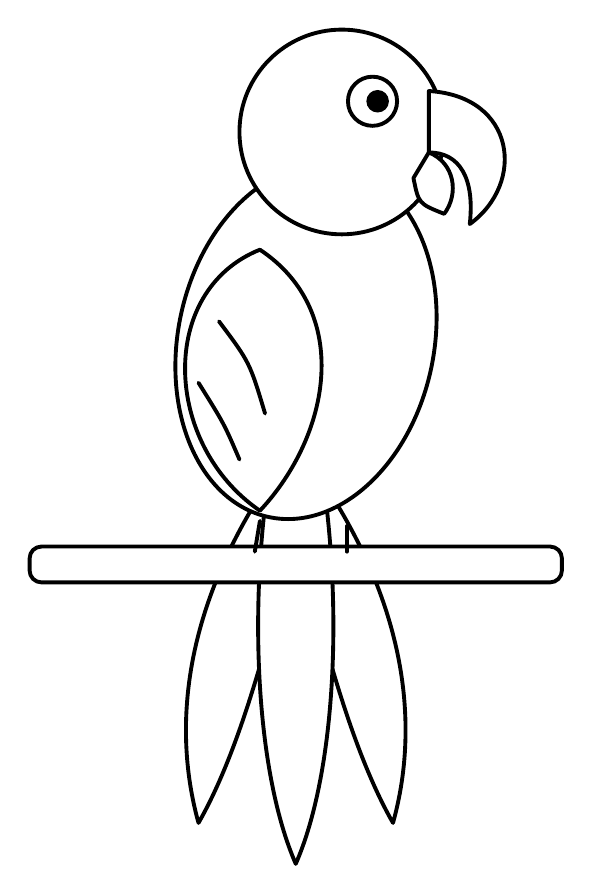
\begin{tikzpicture}[line width=1.4pt, line cap=round, line join=round, scale=1.3]
  % la cola, detrás de todo: tres plumas largas
  \filldraw[fill=white] (-0.35,0.6) .. controls (-1.1,-0.6) and (-1.2,-1.7) .. (-0.95,-2.6)
    .. controls (-0.55,-1.9) and (-0.25,-0.8) .. (0.05,0.5) -- cycle;
  \filldraw[fill=white] (0.35,0.6) .. controls (1.1,-0.6) and (1.2,-1.7) .. (0.95,-2.6)
    .. controls (0.55,-1.9) and (0.25,-0.8) .. (-0.05,0.5) -- cycle;
  \filldraw[fill=white] (-0.3,0.5) .. controls (-0.45,-0.8) and (-0.35,-2.2) .. (0,-3.0)
    .. controls (0.35,-2.2) and (0.45,-0.8) .. (0.3,0.5) -- cycle;
  % la percha
  \filldraw[fill=white, rounded corners=1.5mm] (-2.6,-0.25) rectangle (2.6,0.1);
  % el cuerpo
  \filldraw[fill=white] (0.1,2.1) ellipse [x radius=1.25, y radius=1.75, rotate=-12];
  % el ala
  \filldraw[fill=white] (-0.35,3.0) .. controls (-1.35,2.6) and (-1.3,1.1) .. (-0.35,0.45)
    .. controls (0.35,1.2) and (0.55,2.4) .. (-0.35,3.0) -- cycle;
  \draw (-0.75,2.3) .. controls (-0.45,1.9) .. (-0.3,1.4);
  \draw (-0.95,1.7) .. controls (-0.7,1.3) .. (-0.55,0.95);
  % la cabeza
  \filldraw[fill=white] (0.45,4.15) circle (1.0);
  % el pico, curvo como el de un loro
  \filldraw[fill=white] (1.3,4.55) .. controls (2.15,4.5) and (2.25,3.65) .. (1.7,3.25)
    .. controls (1.75,3.7) and (1.6,3.95) .. (1.3,3.95) -- cycle;
  \filldraw[fill=white] (1.3,3.95) .. controls (1.55,3.85) and (1.6,3.55) .. (1.45,3.35)
    .. controls (1.2,3.45) .. (1.15,3.7) -- cycle;
  % el ojo
  \filldraw[fill=white] (0.75,4.45) circle (0.24);
  \fill (0.8,4.45) circle (0.11);
  % las patas, agarradas a la percha
  \draw (-0.35,0.35) -- (-0.4,0.05); \draw (-0.55,0.1) -- (-0.25,0.1);
  \draw (0.5,0.3) -- (0.5,0.05); \draw (0.35,0.1) -- (0.65,0.1);
\end{tikzpicture}
